\documentclass[11pt, oneside]{article}   	% use "amsart" instead of "article" for AMSLaTeX format
\usepackage{geometry}                		% See geometry.pdf to learn the layout options. There are lots.
\geometry{letterpaper}                   		% ... or a4paper or a5paper or ... 
%\geometry{landscape}                		% Activate for rotated page geometry
%\usepackage[parfill]{parskip}    		% Activate to begin paragraphs with an empty line rather than an indent
\usepackage{graphicx}				% Use pdf, png, jpg, or eps§ with pdflatex; use eps in DVI modesket
								% TeX will automatically convert eps --> pdf in pdflatex		
\usepackage{amssymb}
\usepackage{placeins}

%SetFonts

%SetFonts


\title{Polarimeter Simulation Report for Dr. Herman Marshall}
\author{Adam Theriault-Shay}
\date{June 22, 2016}							% Activate to display a given date or no date

\begin{document}
\maketitle
\section{Introduction}
The primary purpose of the polarimetry simulation is to understand how small imperfections in optical components affect data and imaging. Given the large force satellite observatories undergo during launch, it is important to prepare for any combination of optical imperfections. Space for these imperfections comes from how optical components are bound to their stages, the warping of individual optical components, and slight misalignments.
For the purpose of this simulation, I explored the idealized case in order to establish a control for future variables and testing. The specific trial discussed here is trial 19.
	
\section{Structure}

This simulation is modeled after the lab setup, in which a point source and multi-layer mirror mimic incoming polarized light, and another multi-layer mirror and CCD receive the polarized light. The source of polarized light was then rotated about its axis of propagation to create images for different angles of polarization.
\subsection{Components:}
\begin{enumerate}

\item 2 Multi-layer Mirrors 
\item X-ray Point Source
\item CCD
\end{enumerate}

\subsubsection{MLMirror}
Dimensions: $49mm \times 24mm \times 1mm$\\
Layer thickness varies long the mirror's long axis.

\subsubsection{Point Source}
Photons randomly generated evenly in all directions around the point source. In this simulation, there is a parameter indicating the fraction of the sphere for which the directions are generated. For this simulation the opening angle was 0.05 steradians. This is a measure purely to truncate computation time for irrelevant photons that to not hit the first multi-layer mirror.\\
Source Voltage: 10 kV\\
Source Current: 0.1 mA\\
Source Element: Carbon\\


\subsubsection{CCD}
Dimensions: $24.576mm \times 24.576mm \times 1mm$\\
Pixel Size: $24.576\cdot 10^{-3} mm$

\subsection{Setup}


\subsubsection{Polarized X-Ray Source}
\begin{figure}[h!]
\includegraphics[scale=0.5]{/Users/adamtheriault-shay/Desktop/FIRSTSTAGE.png}
\end{figure}

\newpage
\subsubsection{MLMirror and CCD}
\begin{figure}[h!]
\includegraphics[scale=0.5]{/Users/adamtheriault-shay/Desktop/SECONDSTAGE.png}
\end{figure}

\subsubsection{Simulation Details}
Distance:\\
There was a distance of 10 meters in between the first stage (2.2.1 Polarized X-Ray Source) and the second stage (2.2.2 ML Mirror and CCD).\\
Rotation:\\
With x-axis to the right, y-axis up, and z-out, the first stage was rotated about the x-axis.
Resolution:\\
$6\cdot 10^{6}$ photons per angle. $17 $ Angles (evenly spaced)

\subsection{Adjustments}
The source generated a gaussian energy distribution that had peak reflectivity on one band on the multilayer mirror. In order to maintain an even stream of polarized light throughout the rotation, the mirror had to be shifted so that the peak band of reflectivity intersected with the rotation axis. So the multilayer mirror in the first stage was shifted 6mm in the z+ direction.

\section{Sample Data}

\subsection{Integrated Probability}
\begin{figure}[h!]
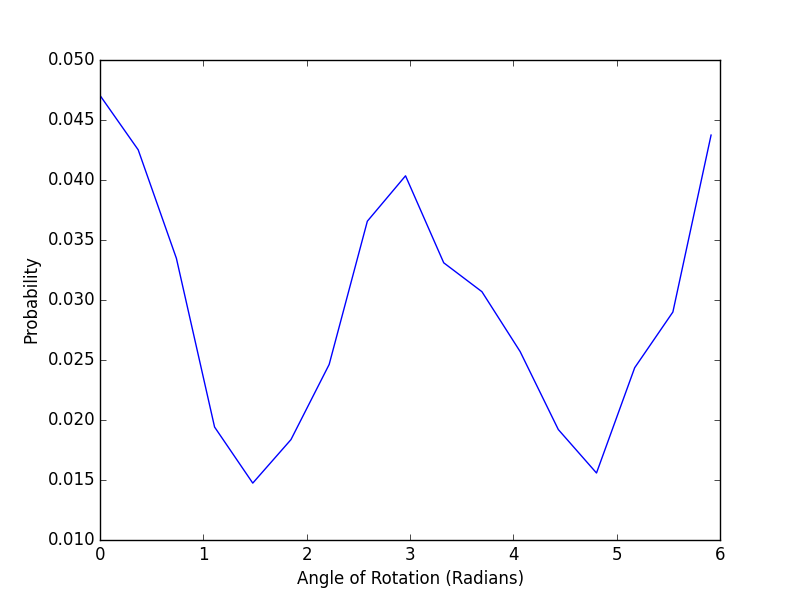
\includegraphics[scale=0.7]{/Users/adamtheriault-shay/Desktop/probability_to_angle.png}
\end{figure}

 \subsection{Probabilities at CCD}
 Here the probability of photons is indicated by their color. They are an HSV gradient from red (low probability) to blue (high probability). The probability scale was consistent across all angles of rotation, with solid red being 0, and solid blue being the maximum probability in the set of all photons across all angles.
 
\newpage
\begin{figure}
\centering
\includegraphics[scale = 0.7]{/Users/adamtheriault-shay/Desktop/CCD/Angle1.png}
\caption{0 rad}
\includegraphics[scale = 0.7]{/Users/adamtheriault-shay/Desktop/CCD/Angle2.png}
\caption{0.37 rad}
\end{figure}

\newpage
\begin{figure}
\includegraphics[scale = 0.7]{/Users/adamtheriault-shay/Desktop/CCD/Angle3.png}
\caption{0.74 rad}
\includegraphics[scale = 0.7]{/Users/adamtheriault-shay/Desktop/CCD/Angle4.png}
\caption{1.11 rad}
\end{figure}


\newpage
\begin{figure}
\includegraphics[scale = 0.7]{/Users/adamtheriault-shay/Desktop/CCD/Angle5.png}
\caption{1.48 rad}
\includegraphics[scale = 0.7]{/Users/adamtheriault-shay/Desktop/CCD/Angle6.png}
\caption{1.85 rad}
\end{figure}

\newpage
\begin{figure}
\includegraphics[scale = 0.7]{/Users/adamtheriault-shay/Desktop/CCD/Angle7.png}
\caption{2.22 rad}
\includegraphics[scale = 0.7]{/Users/adamtheriault-shay/Desktop/CCD/Angle8.png}
\caption{2.59 rad}
\end{figure}

\newpage
\begin{figure}
\includegraphics[scale = 0.7]{/Users/adamtheriault-shay/Desktop/CCD/Angle9.png}
\caption{2.96 rad}
\includegraphics[scale = 0.7]{/Users/adamtheriault-shay/Desktop/CCD/Angle10.png}
\caption{3.32 rad}
\end{figure}

\newpage
\begin{figure}
\includegraphics[scale = 0.7]{/Users/adamtheriault-shay/Desktop/CCD/Angle11.png}
\caption{3.69 rad}
\includegraphics[scale = 0.7]{/Users/adamtheriault-shay/Desktop/CCD/Angle12.png}
\caption{4.06 rad}
\end{figure}

\newpage
\begin{figure}
\includegraphics[scale = 0.7]{/Users/adamtheriault-shay/Desktop/CCD/Angle13.png}
\caption{4.43 rad}
\includegraphics[scale = 0.7]{/Users/adamtheriault-shay/Desktop/CCD/Angle14.png}
\caption{4.80 rad}
\end{figure}

\newpage
\begin{figure}
\includegraphics[scale = 0.7]{/Users/adamtheriault-shay/Desktop/CCD/Angle15.png}
\caption{5.17 rad}
\includegraphics[scale = 0.7]{/Users/adamtheriault-shay/Desktop/CCD/Angle16.png}
\caption{5.54 rad}
\end{figure}

\newpage
\begin{figure}
\includegraphics[scale = 0.7]{/Users/adamtheriault-shay/Desktop/CCD/Angle17.png}
\caption{5.91 rad}
\end{figure}





\FloatBarrier







 \subsection{CCD Probability Distribution}
The following graphs are similar to the previous, except the probabilities are integrated over the photons within each square mm of the CCD.
Blue is maximum (square mm with highest total probability) and minimum is zero.

\begin{figure}
\centering
\includegraphics[scale = 0.7]{/Users/adamtheriault-shay/Desktop/Histogram/Angle1.png}
\caption{0 rad}
\includegraphics[scale = 0.7]{/Users/adamtheriault-shay/Desktop/Histogram/Angle2.png}
\caption{0.37 rad}
\end{figure}

\newpage
\begin{figure}
\includegraphics[scale = 0.7]{/Users/adamtheriault-shay/Desktop/Histogram/Angle3.png}
\caption{0.74 rad}
\includegraphics[scale = 0.7]{/Users/adamtheriault-shay/Desktop/Histogram/Angle4.png}
\caption{1.11 rad}
\end{figure}


\newpage
\begin{figure}
\includegraphics[scale = 0.7]{/Users/adamtheriault-shay/Desktop/Histogram/Angle5.png}
\caption{1.48 rad}
\includegraphics[scale = 0.7]{/Users/adamtheriault-shay/Desktop/Histogram/Angle6.png}
\caption{1.85 rad}
\end{figure}

\newpage
\begin{figure}
\includegraphics[scale = 0.7]{/Users/adamtheriault-shay/Desktop/Histogram/Angle7.png}
\caption{2.22 rad}
\includegraphics[scale = 0.7]{/Users/adamtheriault-shay/Desktop/Histogram/Angle8.png}
\caption{2.59 rad}
\end{figure}

\newpage
\begin{figure}
\includegraphics[scale = 0.7]{/Users/adamtheriault-shay/Desktop/Histogram/Angle9.png}
\caption{2.96 rad}
\includegraphics[scale = 0.7]{/Users/adamtheriault-shay/Desktop/Histogram/Angle10.png}
\caption{3.32 rad}
\end{figure}

\newpage
\begin{figure}
\includegraphics[scale = 0.7]{/Users/adamtheriault-shay/Desktop/Histogram/Angle11.png}
\caption{3.69 rad}
\includegraphics[scale = 0.7]{/Users/adamtheriault-shay/Desktop/Histogram/Angle12.png}
\caption{4.06 rad}
\end{figure}

\newpage
\begin{figure}
\includegraphics[scale = 0.7]{/Users/adamtheriault-shay/Desktop/Histogram/Angle13.png}
\caption{4.43 rad}
\includegraphics[scale = 0.7]{/Users/adamtheriault-shay/Desktop/Histogram/Angle14.png}
\caption{4.80 rad}
\end{figure}

\newpage
\begin{figure}
\includegraphics[scale = 0.7]{/Users/adamtheriault-shay/Desktop/Histogram/Angle15.png}
\caption{5.17 rad}
\includegraphics[scale = 0.7]{/Users/adamtheriault-shay/Desktop/Histogram/Angle16.png}
\caption{5.54 rad}
\end{figure}

\newpage
\begin{figure}
\includegraphics[scale = 0.7]{/Users/adamtheriault-shay/Desktop/Histogram/Angle17.png}
\caption{5.91 rad}
\end{figure}



\end{document}  